% !TEX encoding = UTF-8 Unicode
% !TEX program  = pdflatex
%
% GAT-MARL — Slide thuyết trình
% Beamer, theme: Madrid (hoặc đổi tùy thích)
%

\documentclass[aspectratio=169]{beamer}

% ── Theme ─────────────────────────────────────────────────────────────────────
\usetheme{Madrid}
\usecolortheme{seahorse}

% ── Encoding & Vietnamese ─────────────────────────────────────────────────────
\usepackage[utf8]{inputenc}
\usepackage[vietnamese]{babel}

% ── Packages ──────────────────────────────────────────────────────────────────
\usepackage{amsmath,amssymb}
\usepackage{graphicx}
\usepackage{booktabs}
\usepackage{tikz}
\usepackage{xcolor}
\usepackage{listings}
\usepackage{multicol}

% ── Colors ────────────────────────────────────────────────────────────────────
\definecolor{primary}{RGB}{25, 60, 120}
\definecolor{accent}{RGB}{220, 50, 50}
\definecolor{muted}{RGB}{120, 120, 120}

% ── Metadata ──────────────────────────────────────────────────────────────────
\title[GAT-MARL Traffic Signal Control]{%
  GAT-MARL: Điều phối mạng lưới đèn giao thông đô thị\\
  bằng Multi-Agent Reinforcement Learning\\
  và Graph Attention Network}
\subtitle{Bài tập lớn — Môn Machine Learning, HK2 2025--2026}
\author[Nhóm 13]{Đặng Quang Minh \and Ngô Trọng Hiệp \and Khổng Quang Huy}
\institute[UET-VNU]{Viện Trí tuệ nhân tạo\\Trường Đại học Công nghệ --- ĐHQGHN}
\date{}

% ══════════════════════════════════════════════════════════════════════════════
\begin{document}

% ── TITLE ─────────────────────────────────────────────────────────────────────
\begin{frame}
  \titlepage
  % [GỢI Ý ẢNH] Có thể chèn logo UET hoặc ảnh bản đồ Hà Nội mờ làm background:
  % 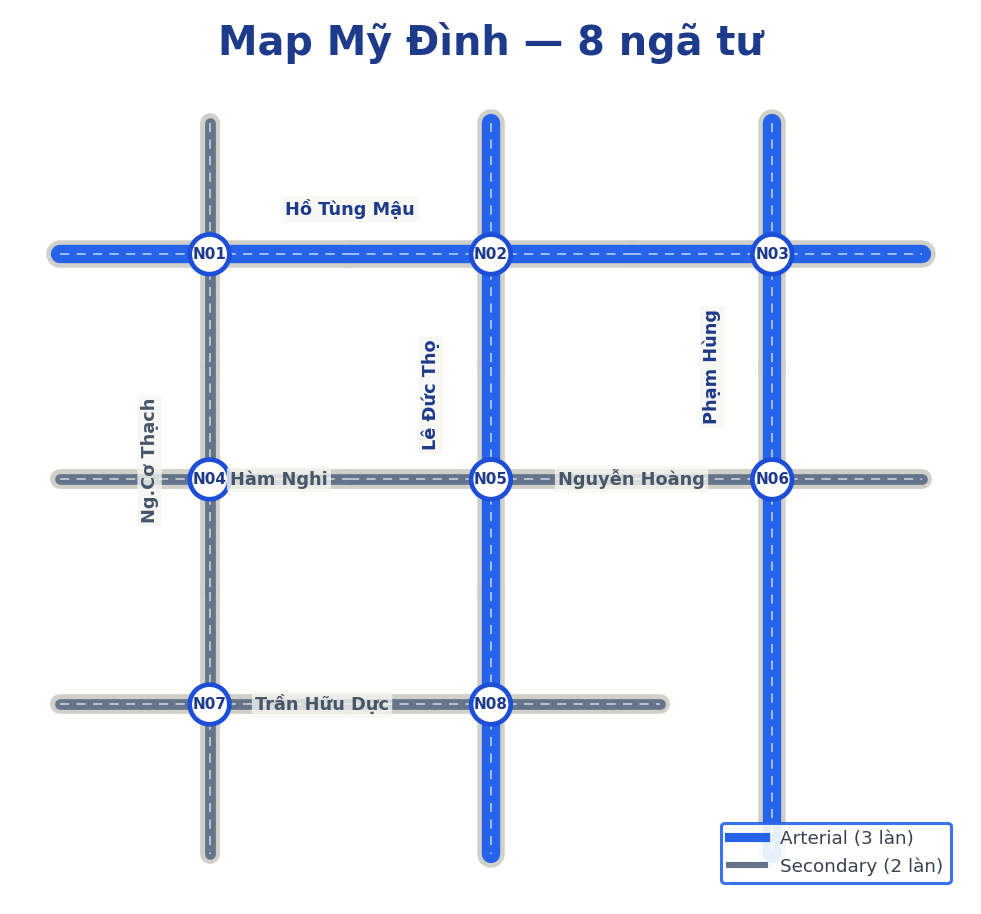
\includegraphics[width=\textwidth]{imgs/map_mydinh.png}
\end{frame}

% ── OUTLINE ───────────────────────────────────────────────────────────────────
\begin{frame}{Nội dung trình bày}
  \tableofcontents
\end{frame}

% ══════════════════════════════════════════════════════════════════════════════
\section{Giới thiệu bài toán}
% ══════════════════════════════════════════════════════════════════════════════

\begin{frame}{Vấn đề: Đèn giao thông truyền thống}
  \begin{columns}
    \column{0.55\textwidth}
      \textbf{Hạn chế của hệ thống cố định:}
      \begin{itemize}
        \item Chu kỳ cứng nhắc, không phản ứng với lưu lượng thực tế
        \item Mỗi ngã tư hoạt động độc lập, không phối hợp
        \item Ùn tắc cục bộ lan sang toàn mạng
      \end{itemize}
      \vspace{0.5em}
      \textbf{Mục tiêu:} Hệ thống \textit{adaptive} tối thiểu hóa\\
      thời gian chờ và tăng lưu lượng thông qua.

    \column{0.45\textwidth}
      % [GỢI Ý ẢNH] Ảnh chụp thực tế tắc đường Hà Nội hoặc ảnh vệ tinh
      % giao lộ khu vực Mỹ Đình:
      \begin{center}
        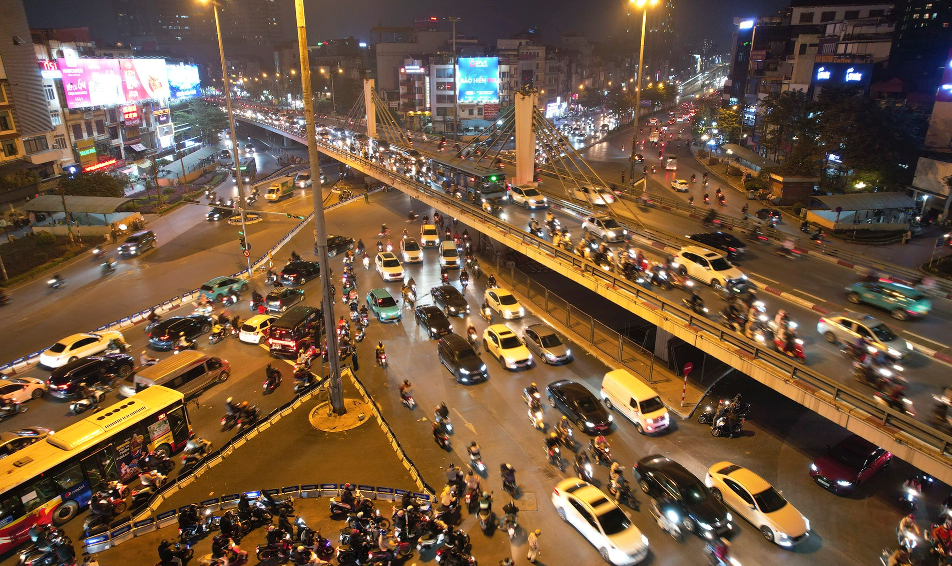
\includegraphics[width=\linewidth]{imgs/un-tac-ha-noi.png}
        % \textit{[Ảnh: tắc đường thực tế / bản đồ khu vực Mỹ Đình]}
      \end{center}
  \end{columns}
\end{frame}

% ── Mô hình hóa bài toán ──────────────────────────────────────────────────────
\begin{frame}{Mô hình hóa: Dec-POMDP}
  \begin{block}{Decentralized Partially Observable MDP}
    Mỗi ngã tư $i$ là một \textbf{agent} quyết định pha đèn dựa trên \textit{quan sát cục bộ}.
  \end{block}

  \vspace{0.4em}
  \begin{columns}
    \column{0.5\textwidth}
      \begin{tabular}{ll}
        \toprule
        \textbf{Thành phần} & \textbf{Định nghĩa} \\
        \midrule
        Agents $N$ & 8 ngã tư (Mỹ Đình) \\
        Observation & Queue, density, phase, $\Delta t$ \\
        Action & Keep / Switch pha \\
        Reward & $-(\alpha\hat{w}_i + \beta\hat{p}_i)\times S$ \\
        \bottomrule
      \end{tabular}

    \column{0.5\textwidth}
      \textbf{Thách thức — Non-stationarity:}\\
      Khi agents đồng thời cập nhật policy, môi trường
      trở nên non-stationary từ góc nhìn mỗi agent
      $\Rightarrow$ Independent Q-Learning không hội tụ.
  \end{columns}
\end{frame}

% ══════════════════════════════════════════════════════════════════════════════
\section{Kiến trúc GAT-MARL}
% ══════════════════════════════════════════════════════════════════════════════

\begin{frame}{Kiến trúc mô hình GAT-MARL}
  \begin{columns}
    \column{0.45\textwidth}
      \textbf{3 module dùng chung trọng số:}
      \begin{enumerate}
        \item \textbf{Local Encoder} (MLP)\\
              $\text{obs}_i \to \mathbf{h}_i \in \mathbb{R}^{64}$
        \item \textbf{GAT Layer} (4 heads)\\
              $\mathbf{h}_i \to \mathbf{h}'_i$ (aggregate neighbors)
        \item \textbf{Q-head} (MLP)\\
              $\mathbf{h}'_i \to Q(\text{keep}),\, Q(\text{switch})$
      \end{enumerate}
      \vspace{0.4em}
      \textit{Parameter sharing:} toàn bộ $N$ agents\\
      dùng chung 1 bộ trọng số.

    \column{0.55\textwidth}
      \begin{center}
        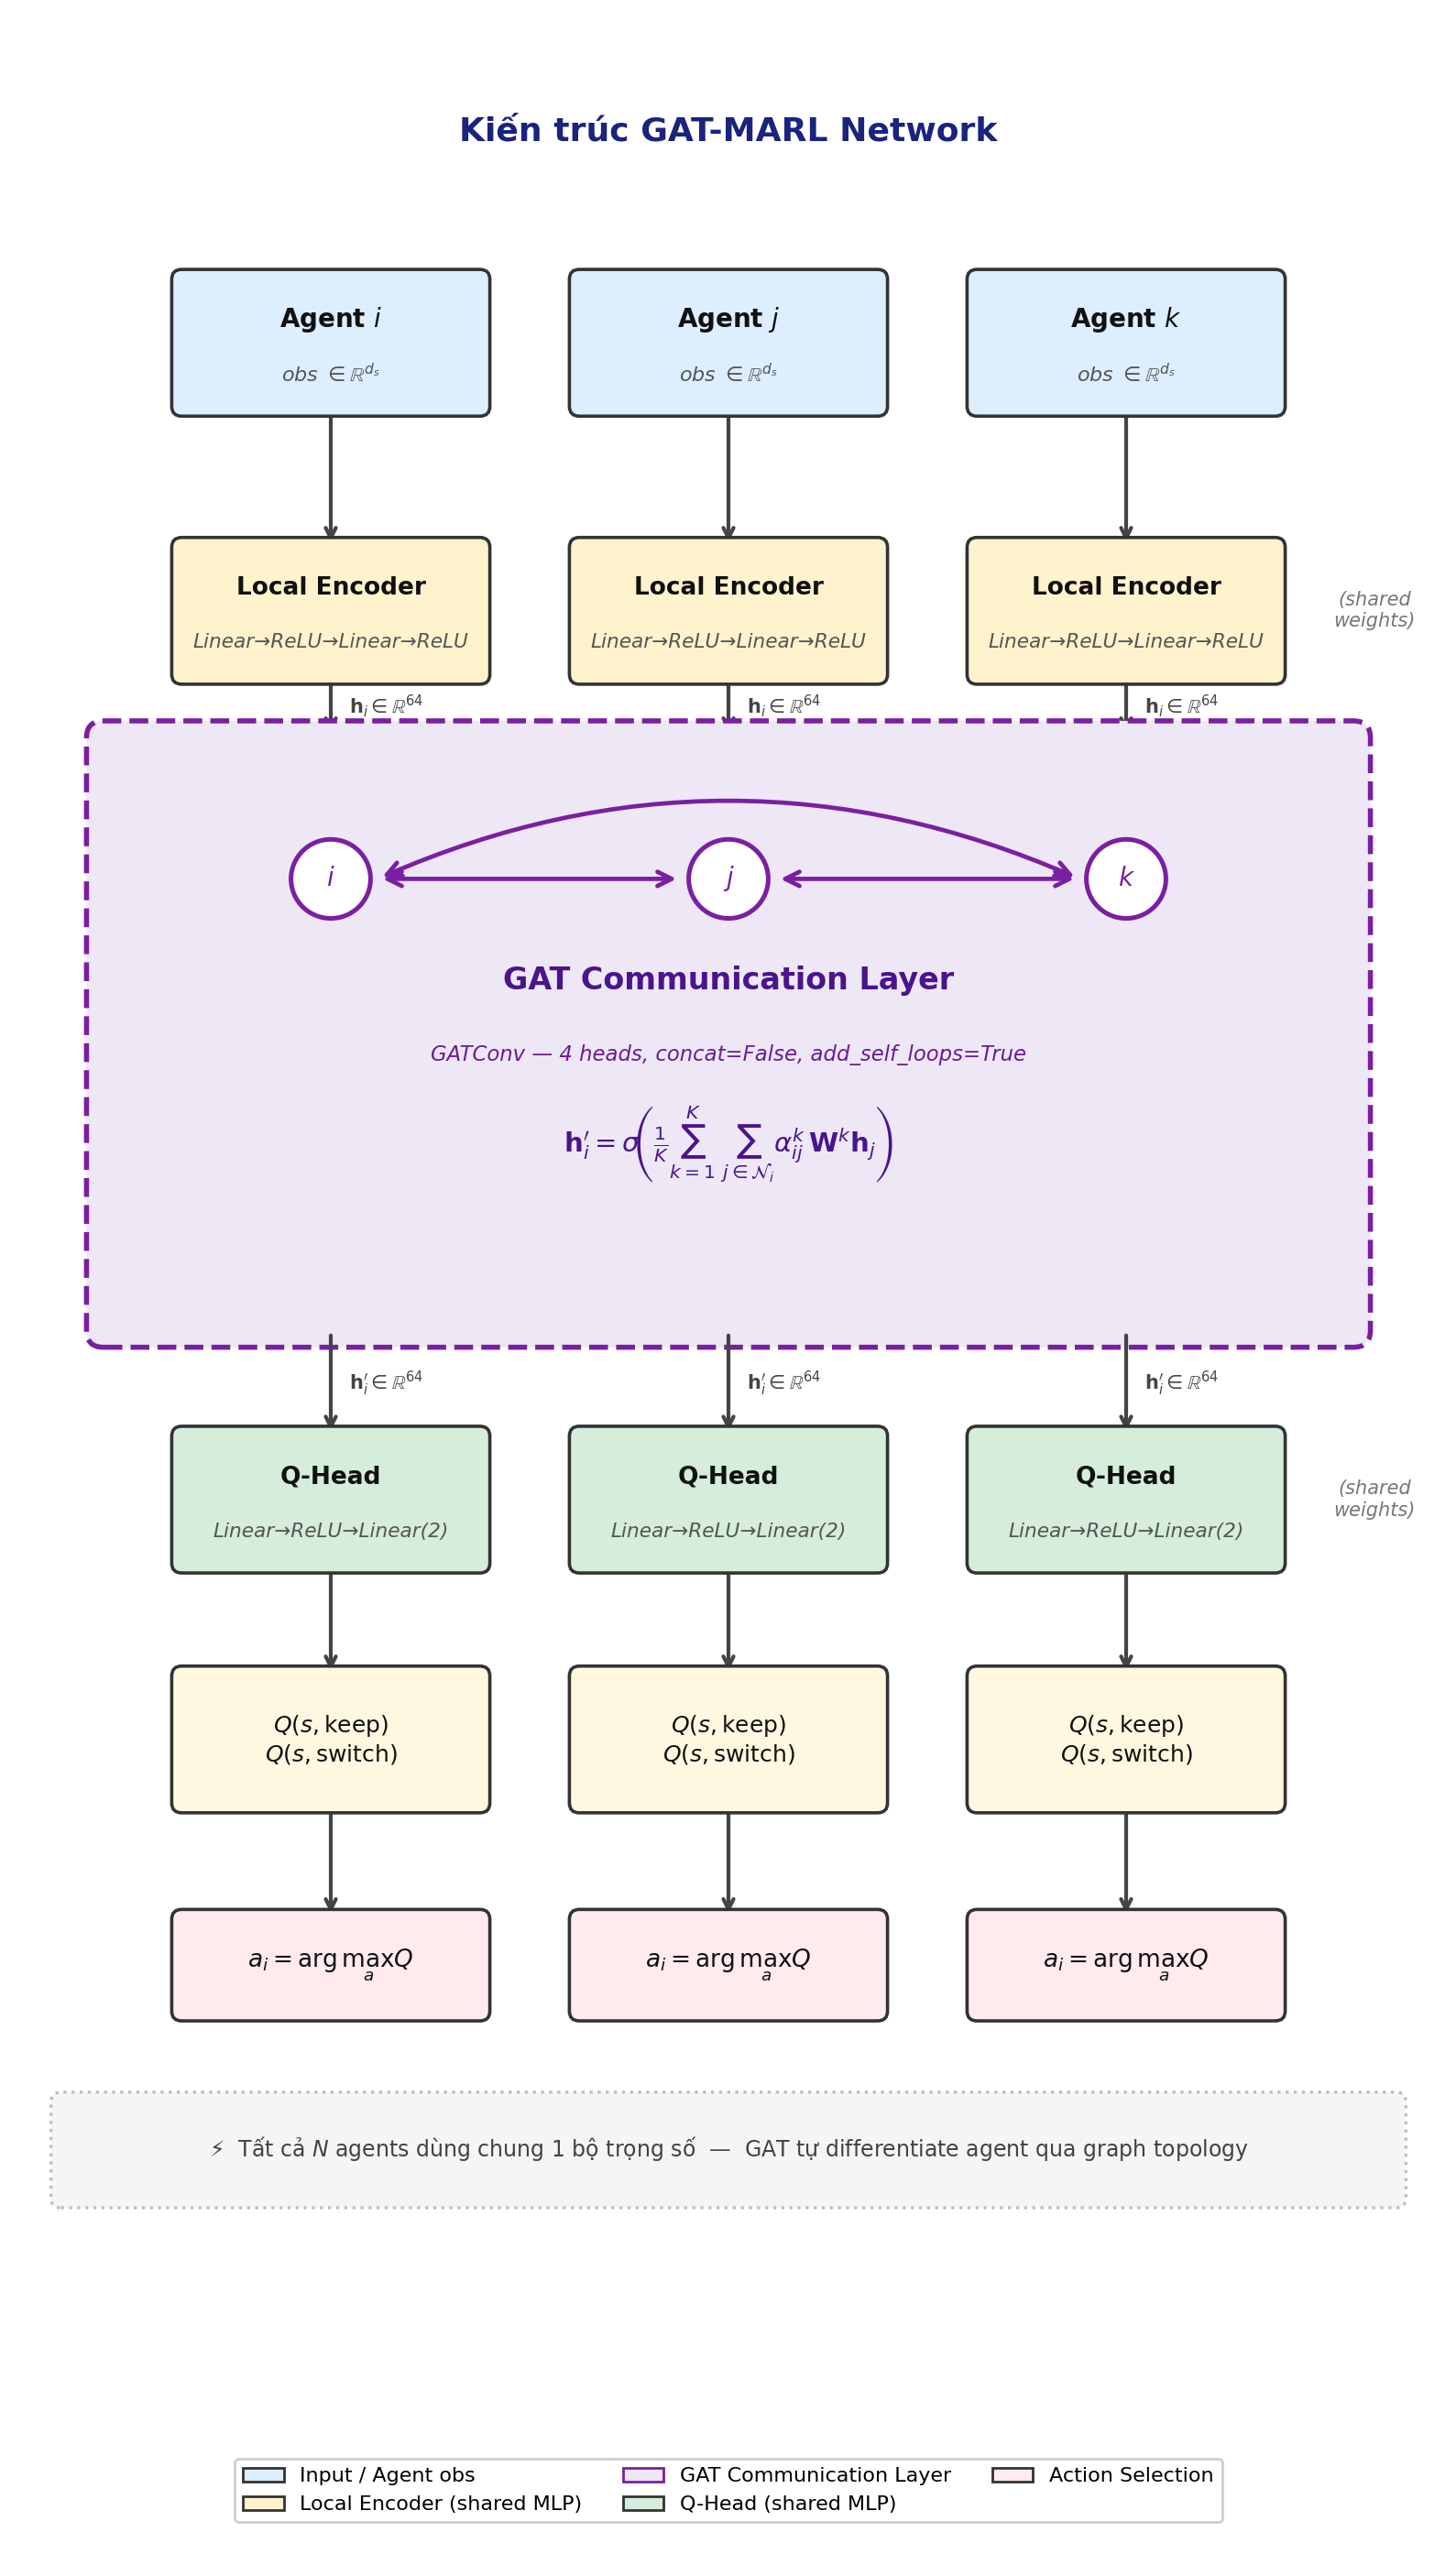
\includegraphics[width=\linewidth,height=0.72\textheight,keepaspectratio]{imgs/gat_marl_architecture.png}
      \end{center}
  \end{columns}
\end{frame}

% ── GAT attention ─────────────────────────────────────────────────────────────
\begin{frame}{Graph Attention Network — Cơ chế giao tiếp}
  \begin{columns}
    \column{0.5\textwidth}
      Hệ số attention giữa agent $i$ và neighbor $j$:
      \begin{equation*}
        \alpha_{ij} = \frac{\exp(\text{LReLU}(e_{ij}))}
                           {\sum_{k \in \mathcal{N}_i} \exp(\text{LReLU}(e_{ik}))}
      \end{equation*}
      \vspace{0.3em}
      \textbf{Ưu điểm:}
      \begin{itemize}
        \item Không cần edge weights định trước
        \item Mức độ ảnh hưởng học được động theo traffic
        \item \texttt{concat=False} $\Rightarrow$ output giữ nguyên 64 chiều
      \end{itemize}

    \column{0.5\textwidth}
      \begin{center}
        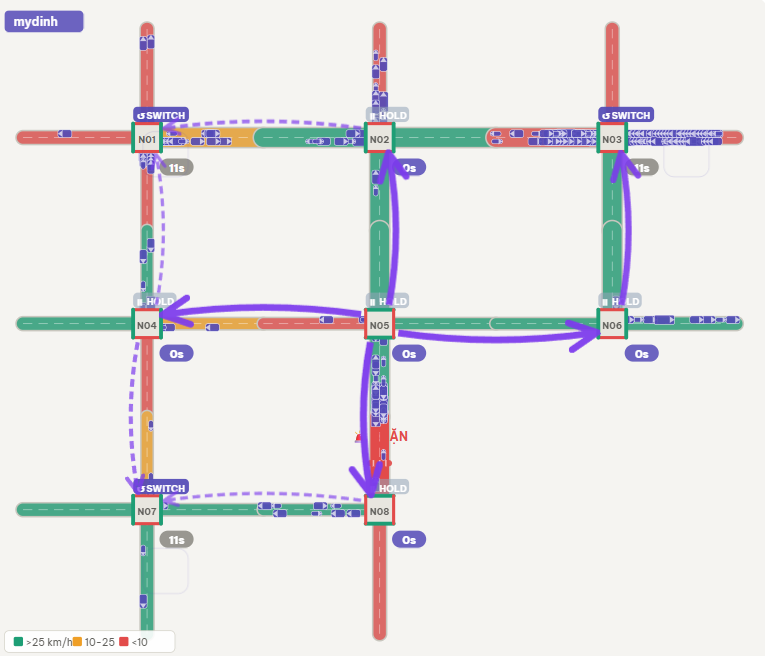
\includegraphics[width=\linewidth,height=0.65\textheight,keepaspectratio]{imgs/attention_mydinh.png}\\
        \small Attention heatmap tại giờ cao điểm
      \end{center}
  \end{columns}
\end{frame}

% ── Reward ────────────────────────────────────────────────────────────────────
\begin{frame}{Reward Function — Hybrid Waiting Time + Pressure}
  \begin{equation*}
    r_i = -\!\left(\alpha \cdot \hat{w}_i + \beta \cdot \hat{p}_i\right) \times S
  \end{equation*}

  \vspace{0.3em}
  \begin{columns}
    \column{0.5\textwidth}
      \textbf{Tại sao cần normalize?}
      \begin{itemize}
        \item Không normalize: tỉ lệ thực tế \textbf{98:2}\\
              (pressure bị triệt tiêu hoàn toàn)
        \item Có normalize: tỉ lệ thực tế \textbf{71:29}\\
              ($\approx \alpha{:}\beta = 70{:}30$ như thiết kế)
      \end{itemize}

    \column{0.5\textwidth}
      \begin{block}{Shared reward (GAT-MARL)}
        $r_i^{\text{train}} = 0.7\cdot r_i + 0.3\cdot \bar{r}$\\[0.3em]
        \small Giữ 70\% tín hiệu per-agent để Q-values\\
        không collapse + 30\% global mean để cooperative.
      \end{block}
  \end{columns}

  % [GỢI Ý ẢNH] Có thể thêm biểu đồ bar chart minh hoạ
  % tỉ lệ 98:2 vs 71:29 bằng TikZ hoặc ảnh matplotlib
\end{frame}

% ══════════════════════════════════════════════════════════════════════════════
\section{Phương pháp training}
% ══════════════════════════════════════════════════════════════════════════════

\begin{frame}{Parallel Training — Ape-X Style}
  \begin{columns}
    \column{0.45\textwidth}
      \textbf{Fixed-role epsilon workers:}
      \begin{equation*}
        \varepsilon_k = \varepsilon_{\max} - \frac{(\varepsilon_{\max}-\varepsilon_{\min})\cdot k}{K-1}
      \end{equation*}
      \begin{itemize}
        \item $k=0$: $\varepsilon=1.0$ — explorer, phủ rộng state space
        \item $k=K-1$: $\varepsilon=0.1$ — near-greedy, on-policy data
      \end{itemize}
      \vspace{0.3em}
      Buffer \textit{luôn} đa dạng từ đầu đến cuối training.

    \column{0.55\textwidth}
      \begin{center}
        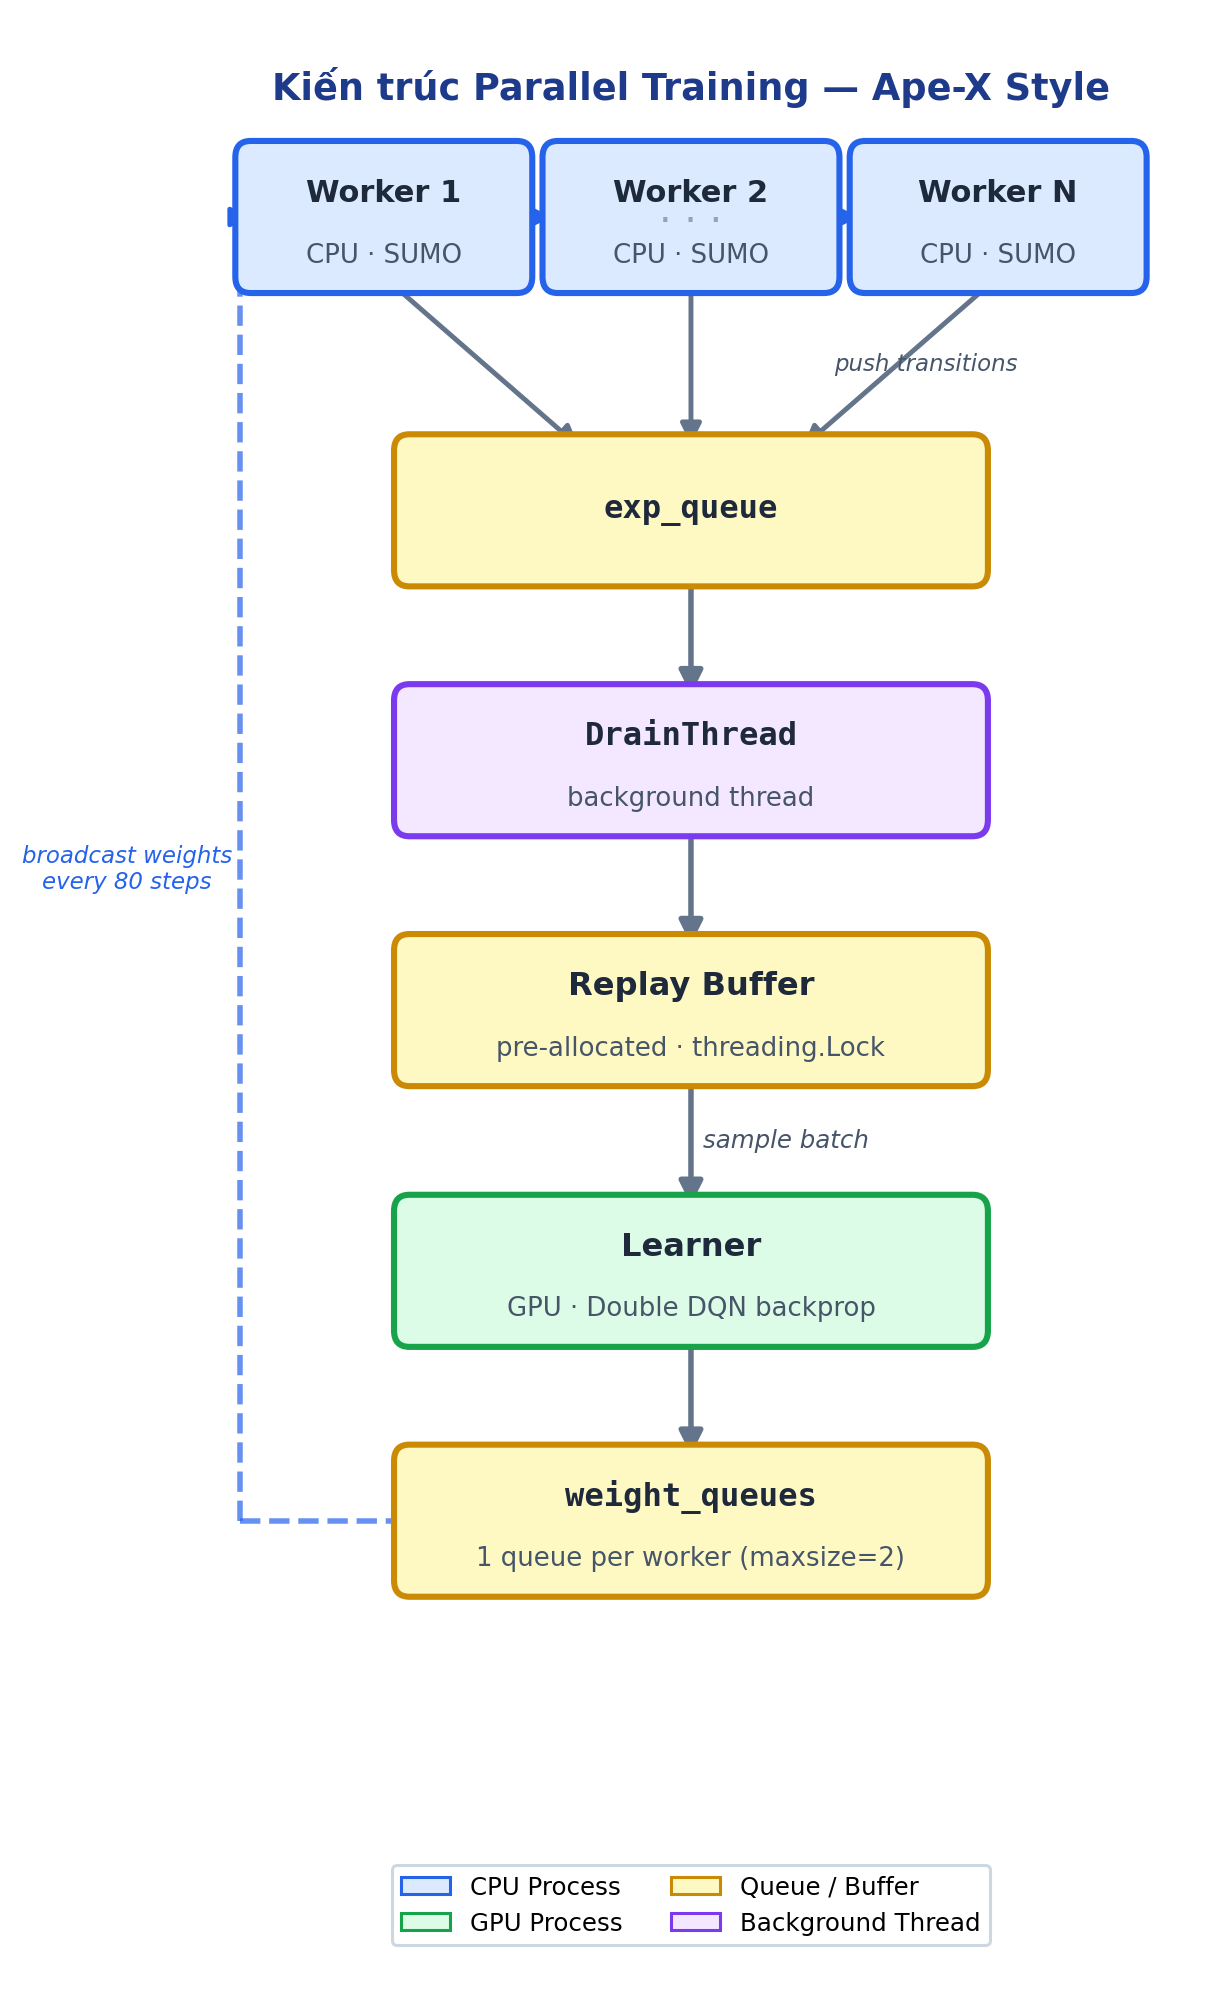
\includegraphics[width=\linewidth,height=0.72\textheight,keepaspectratio]{imgs/apex_diagram.png}
      \end{center}
  \end{columns}
\end{frame}

% ── Fine-tuning ───────────────────────────────────────────────────────────────
\begin{frame}{2-Phase Fine-tuning — Transfer Learning}
  \begin{columns}
    \column{0.5\textwidth}
      \begin{block}{Phase 1 — Freeze GAT (20 ep đầu)}
        GAT layer đóng băng, chỉ Q-head cập nhật.\\
        \small GAT đã học \textit{graph topology knowledge} có tính tổng quát cao.
      \end{block}
      \vspace{0.4em}
      \begin{block}{Phase 2 — Unfreeze toàn bộ}
        Fine-tune toàn bộ với LR thấp (đã qua warmup).
      \end{block}
      \vspace{0.4em}
      \textbf{IDQN:} không có module tách biệt\\
      $\Rightarrow$ phải train lại từ đầu khi đổi map.

    \column{0.5\textwidth}
      % [GỢI Ý ẢNH] Diagram minh hoạ: 2 phase với mũi tên
      % "Freeze" → "Unfreeze", hoặc ảnh checkpoint flow.
      % Có thể vẽ bằng TikZ:
      \begin{center}
            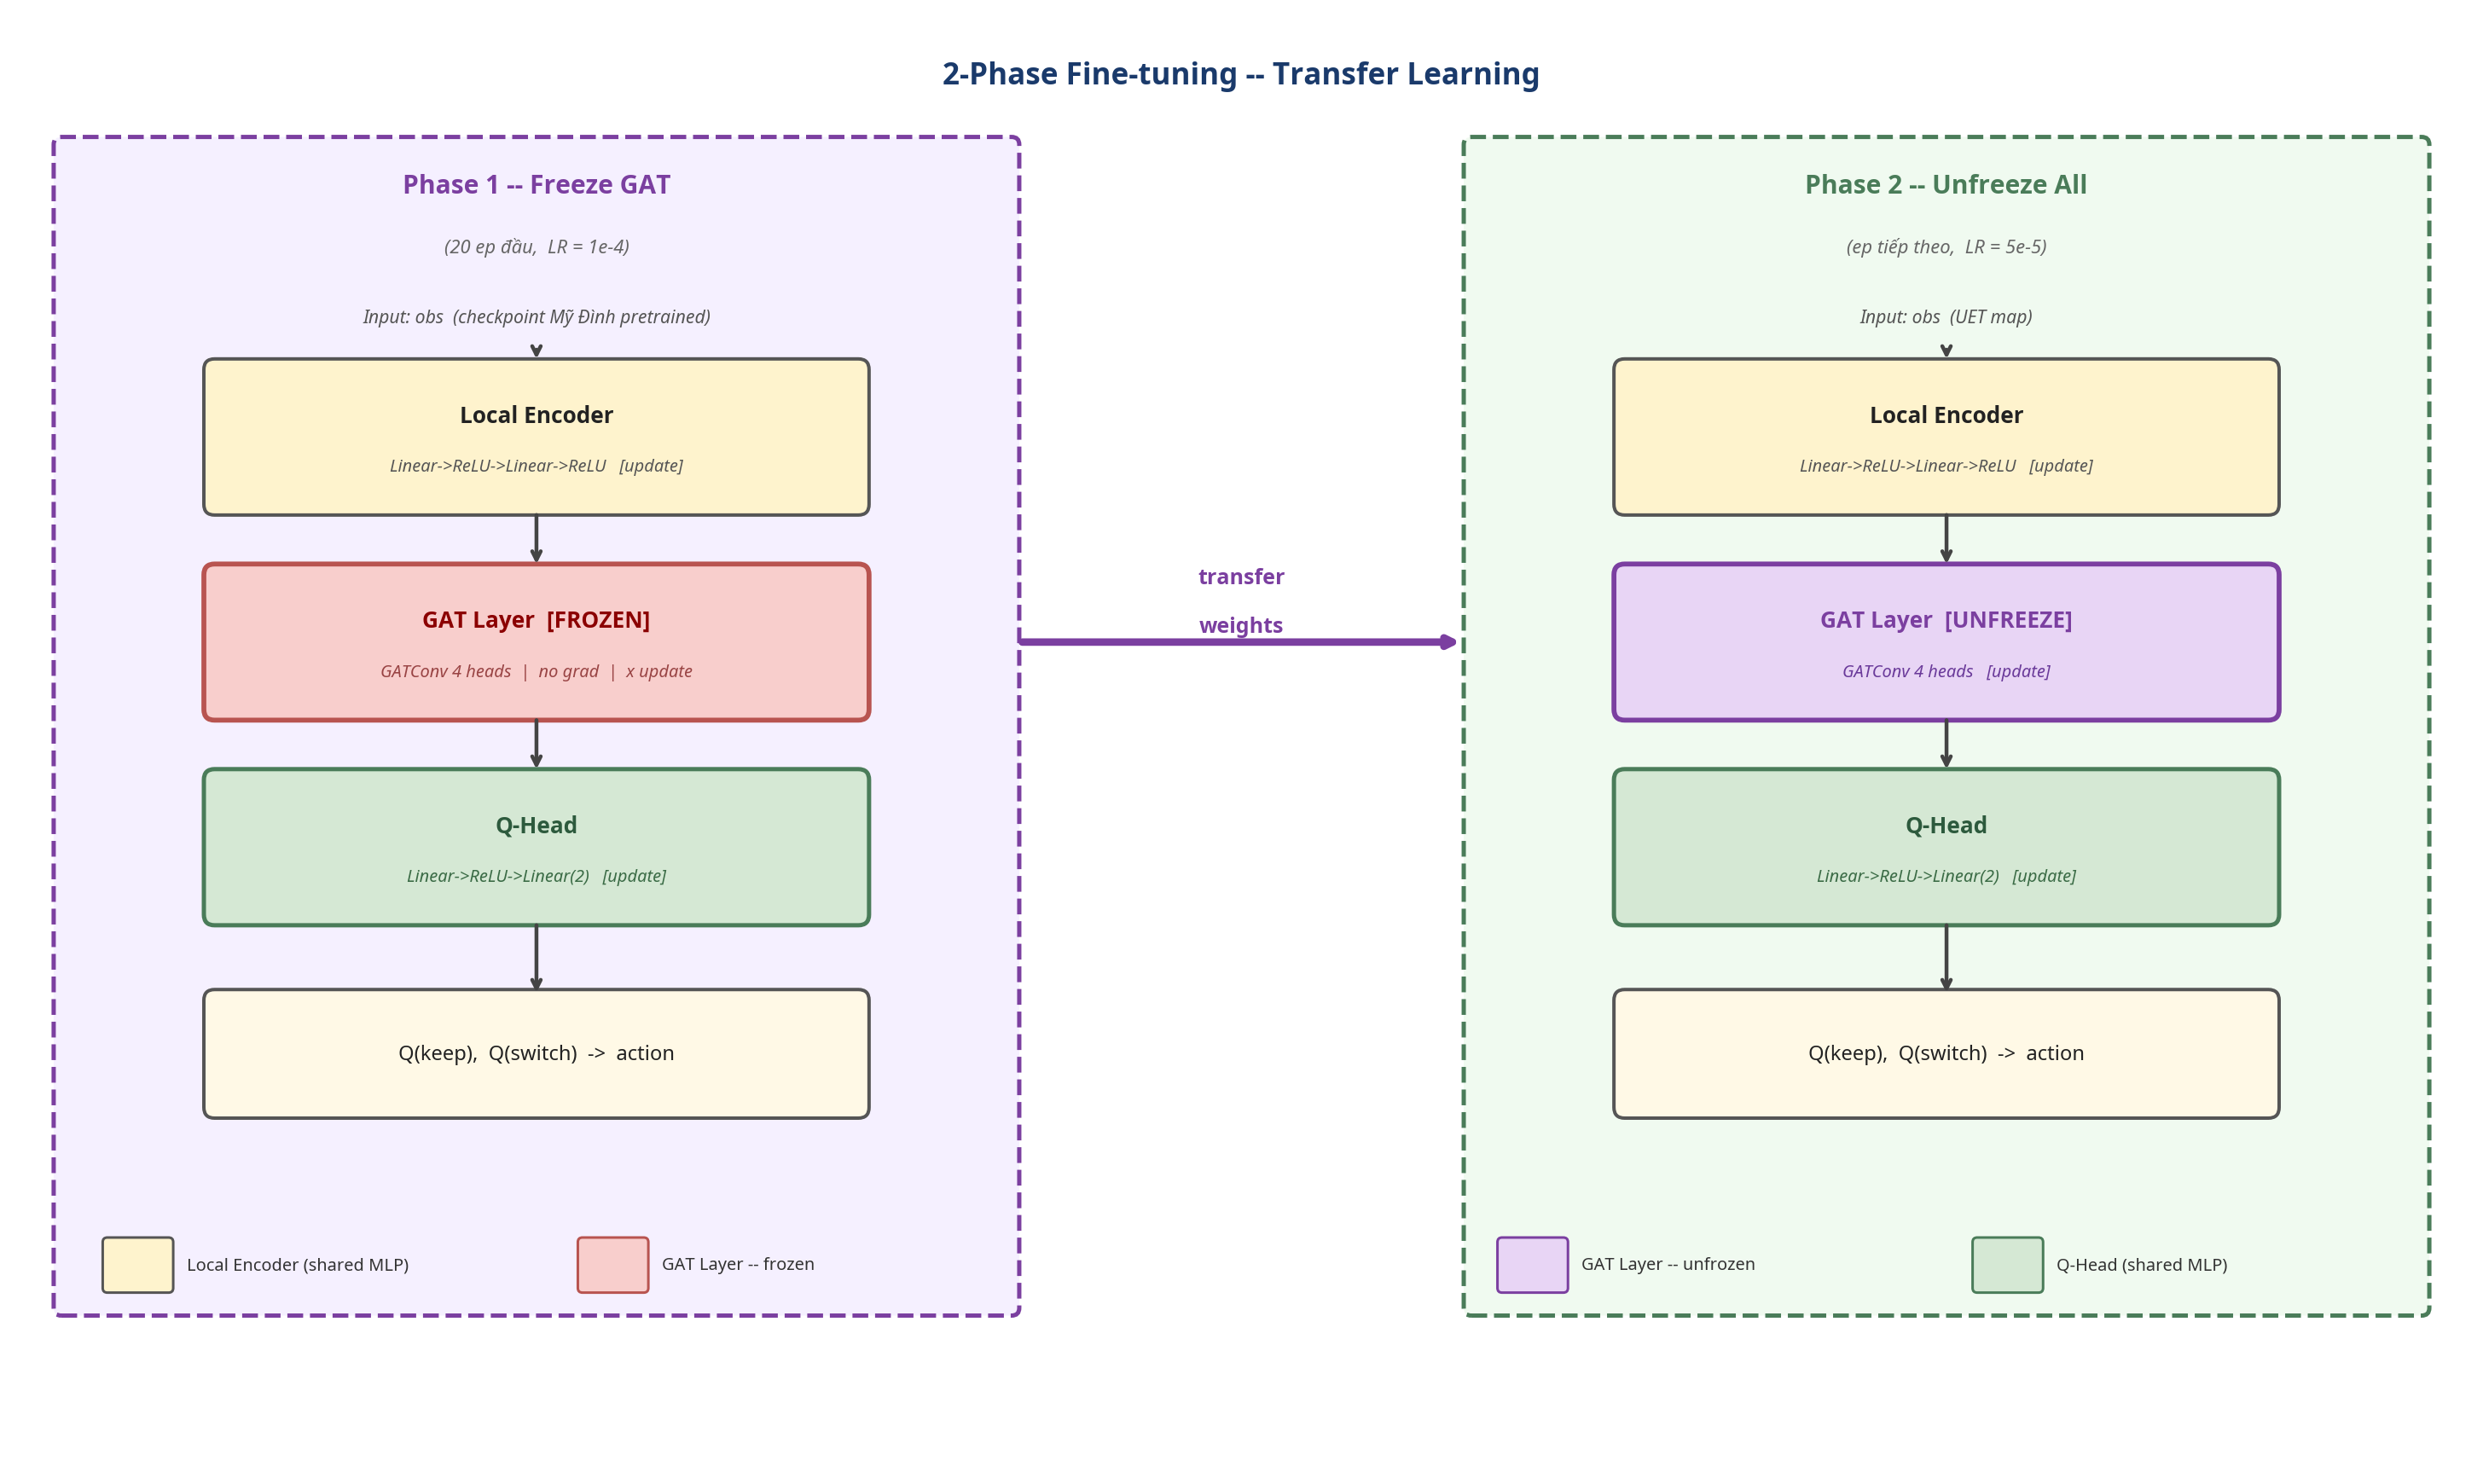
\includegraphics[width=\linewidth]{imgs/finetune_diagram.png}
      \end{center}
  \end{columns}
\end{frame}

% ══════════════════════════════════════════════════════════════════════════════
\section{Môi trường thực nghiệm}
% ══════════════════════════════════════════════════════════════════════════════

\begin{frame}{Môi trường mô phỏng SUMO}
  \begin{columns}
    \column{0.5\textwidth}
      \textbf{Hai mạng lưới thực tế tại Hà Nội:}
      \begin{itemize}
        \item \textbf{Mỹ Đình} — 8 ngã tư\\
              Arterial: Hồ Tùng Mậu, Lê Đức Thọ, Phạm Hùng\\
              Secondary: Hàm Nghi, Nguyễn Hoàng, \ldots
        \item \textbf{UET} — 15 ngã tư\\
              Phức tạp hơn, dùng để kiểm chứng transfer learning
      \end{itemize}
      \vspace{0.4em}
      \textbf{Cấu hình:} 1800s/episode, $\Delta t = 5$s,\\
      3 kịch bản lưu lượng: sáng / chiều / đêm.

    \column{0.5\textwidth}
      % [GỢI Ý ẢNH] Hai ảnh topology cạnh nhau:
      \begin{center}
        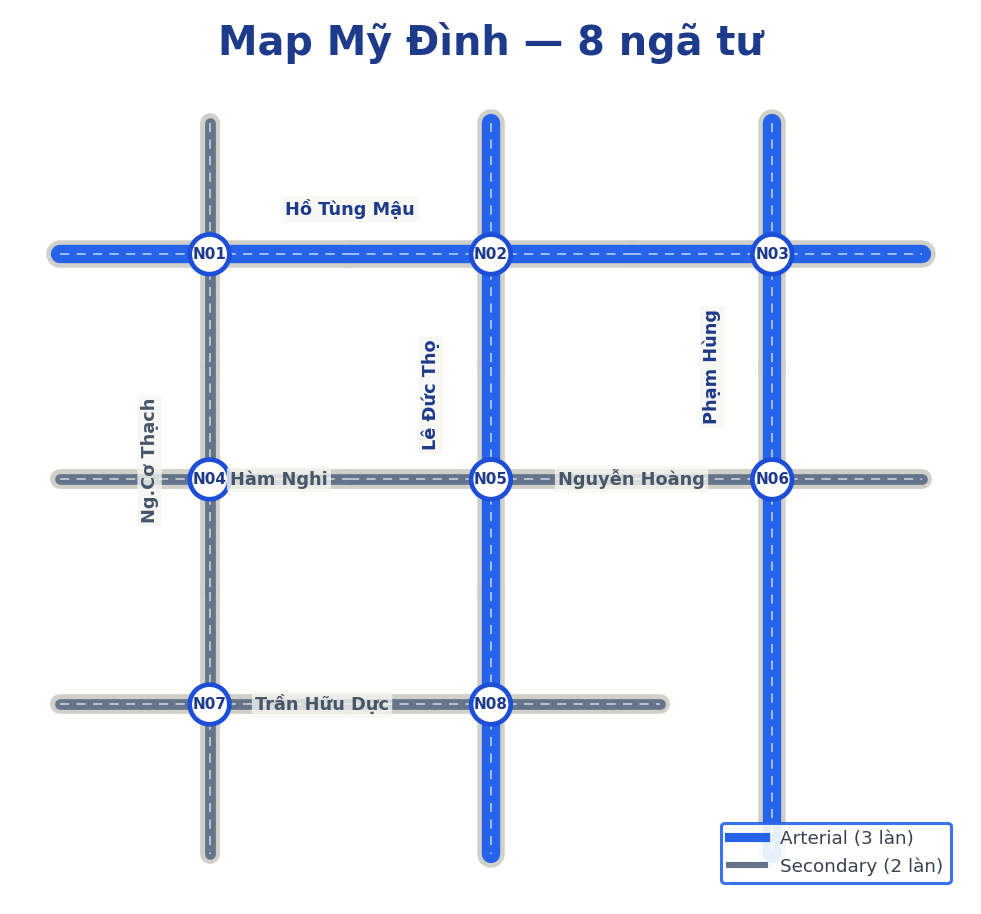
\includegraphics[width=0.48\linewidth]{imgs/map_mydinh.png}
        \hfill
        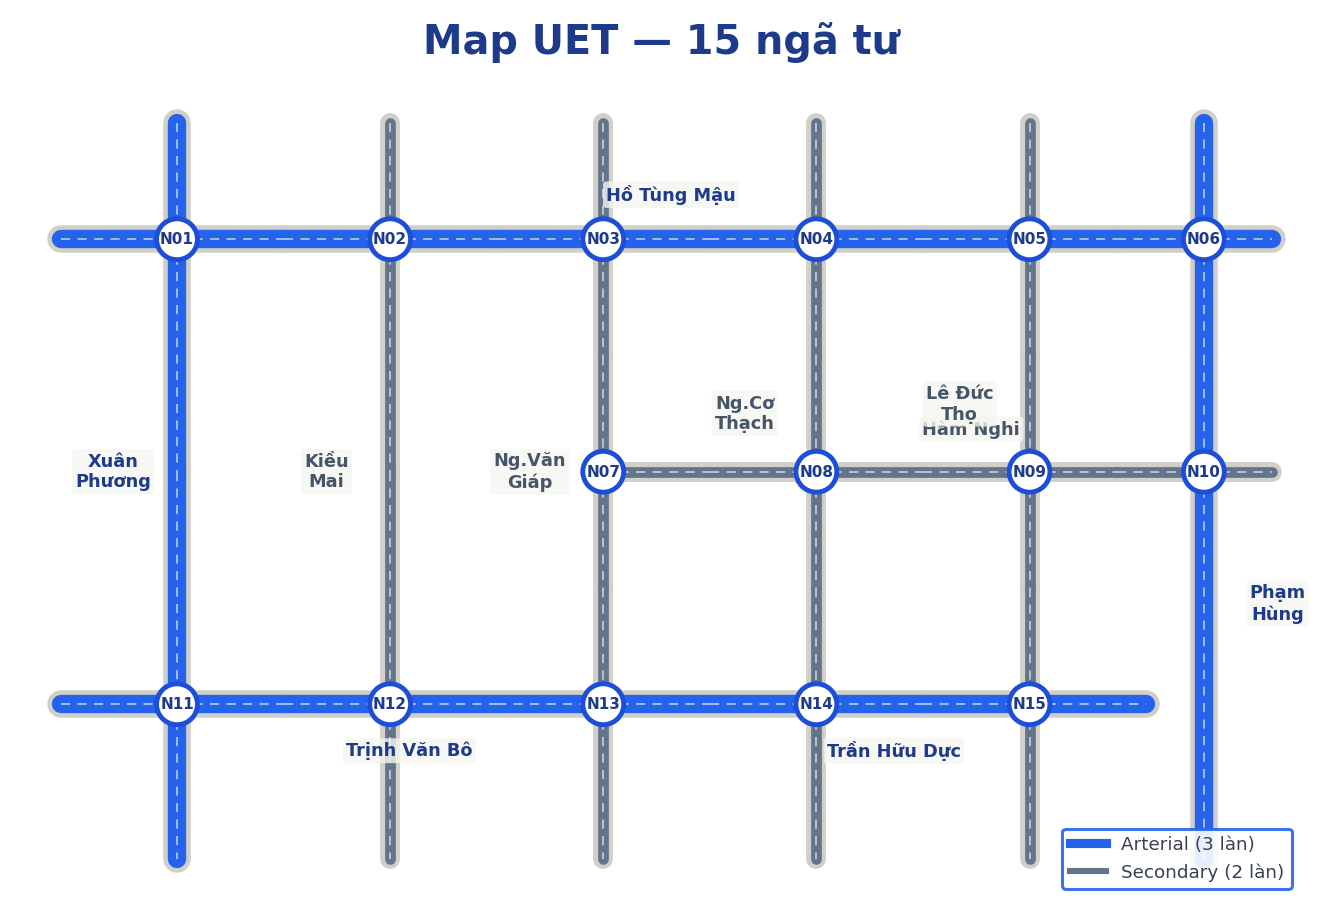
\includegraphics[width=0.48\linewidth]{imgs/map_uet.png}\\
        \small Mỹ Đình (8 ngã tư) \hfill UET (15 ngã tư)
      \end{center}
  \end{columns}
\end{frame}

% ══════════════════════════════════════════════════════════════════════════════
\section{Kết quả thực nghiệm}
% ══════════════════════════════════════════════════════════════════════════════

\begin{frame}{Kết quả — Map Mỹ Đình (500 episodes)}
  \begin{columns}
    \column{0.55\textwidth}
      \begin{center}
        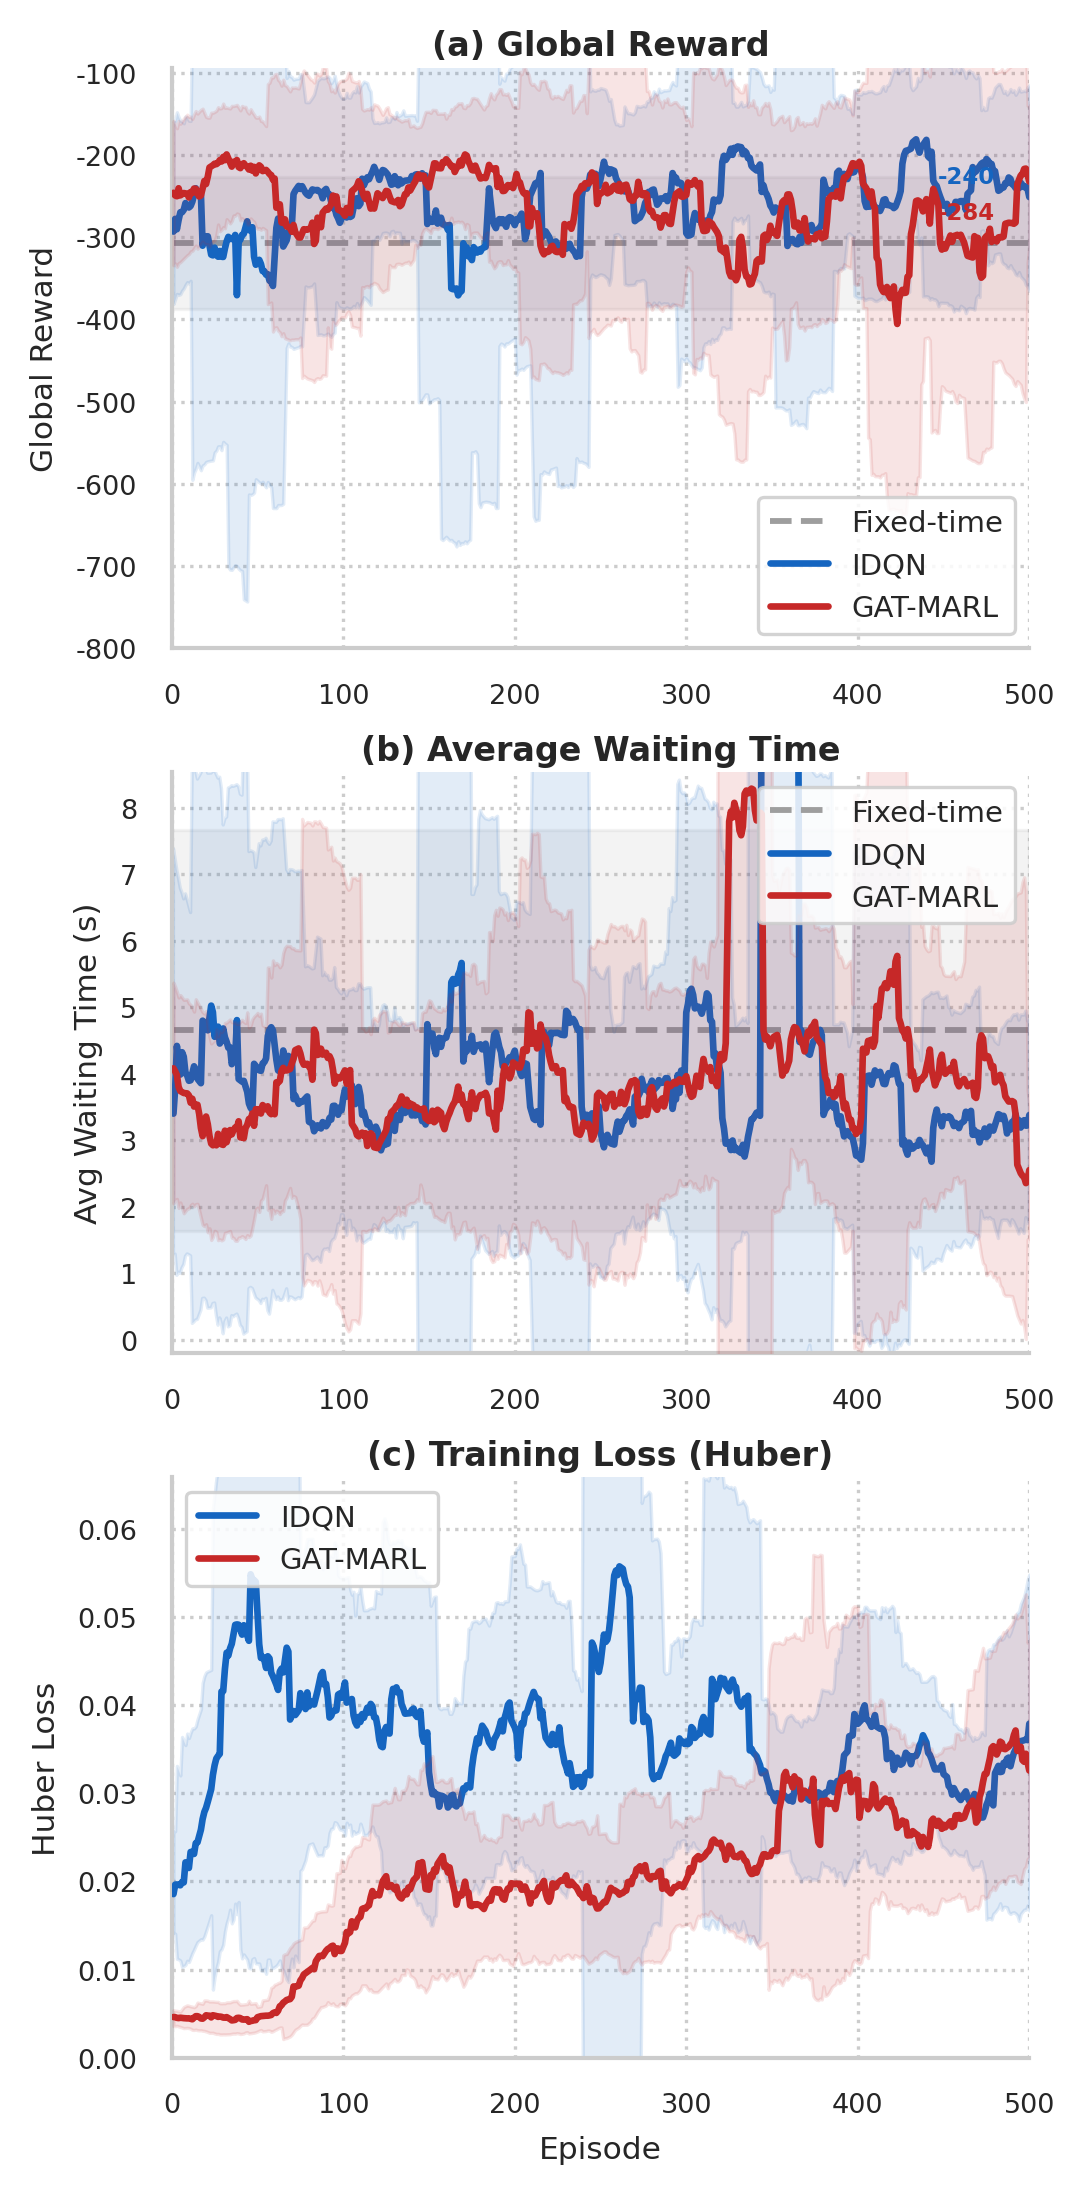
\includegraphics[width=\linewidth,height=0.7\textheight,keepaspectratio]{imgs/learning_curves_mydinh.png}
      \end{center}

    \column{0.45\textwidth}
      \small
      \begin{tabular}{lccc}
        \toprule
        \textbf{Metric} & \textbf{Fixed} & \textbf{IDQN} & \textbf{GAT} \\
        \midrule
        Reward $\uparrow$ & $-364$ & $\mathbf{-260}$ & $-340$ \\
        Wait (s) $\downarrow$ & $5.18$ & $\mathbf{3.99}$ & $4.46$ \\
        Speed $\uparrow$ & $18.9$ & $\mathbf{21.9}$ & $18.7$ \\
        \bottomrule
      \end{tabular}
      \vspace{0.5em}

      \begin{alertblock}{Lưu ý throughput}
        \small Fixed-time có throughput cao hơn vì SUMO
        inject xe đều đặn hơn — không phản ánh
        chất lượng điều phối thực sự.
      \end{alertblock}
  \end{columns}
\end{frame}

% ── Transfer sang UET ─────────────────────────────────────────────────────────
\begin{frame}{Transfer Learning — Mỹ Đình $\to$ UET}
  \begin{columns}
    \column{0.5\textwidth}
      \begin{tabular}{lccc}
        \toprule
        \textbf{Phương pháp} & \textbf{Conv.} & \textbf{Reward} \\
        \midrule
        GAT-MARL (finetune) & \textbf{20 ep} & $-648 \pm 320$ \\
        IDQN (scratch)      & 25 ep          & $-689 \pm 325$ \\
        Fixed-time          & ---            & $-768 \pm 301$ \\
        \bottomrule
      \end{tabular}
      \vspace{0.5em}

      \small $^*$Conv.: số episodes đạt rolling-5 mean $\geq -569$

      \vspace{0.4em}
      \textbf{GAT-MARL học nhanh hơn và reward cuối tốt hơn}
      nhờ tái sử dụng graph topology knowledge từ Mỹ Đình.

    \column{0.5\textwidth}
      \begin{center}
        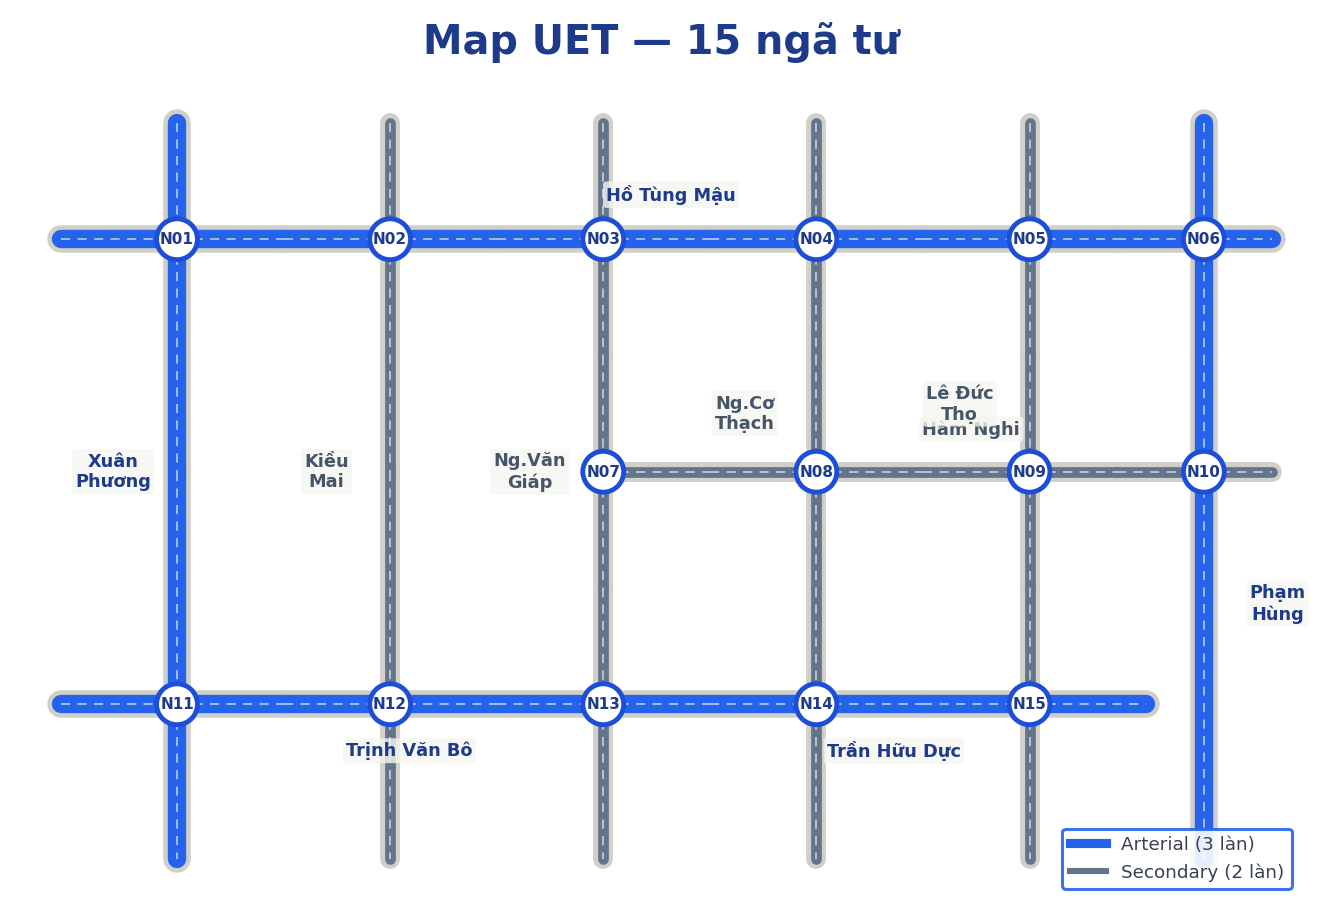
\includegraphics[width=\linewidth,height=0.6\textheight,keepaspectratio]{imgs/map_uet.png}\\
        \small Map UET — 15 ngã tư
      \end{center}
  \end{columns}
\end{frame}

% ── Dashboard ─────────────────────────────────────────────────────────────────
\begin{frame}{Dashboard Real-time}
  % [GỢI Ý ẢNH] Screenshot dashboard live demo — 3 panels song song:
  \begin{center}
    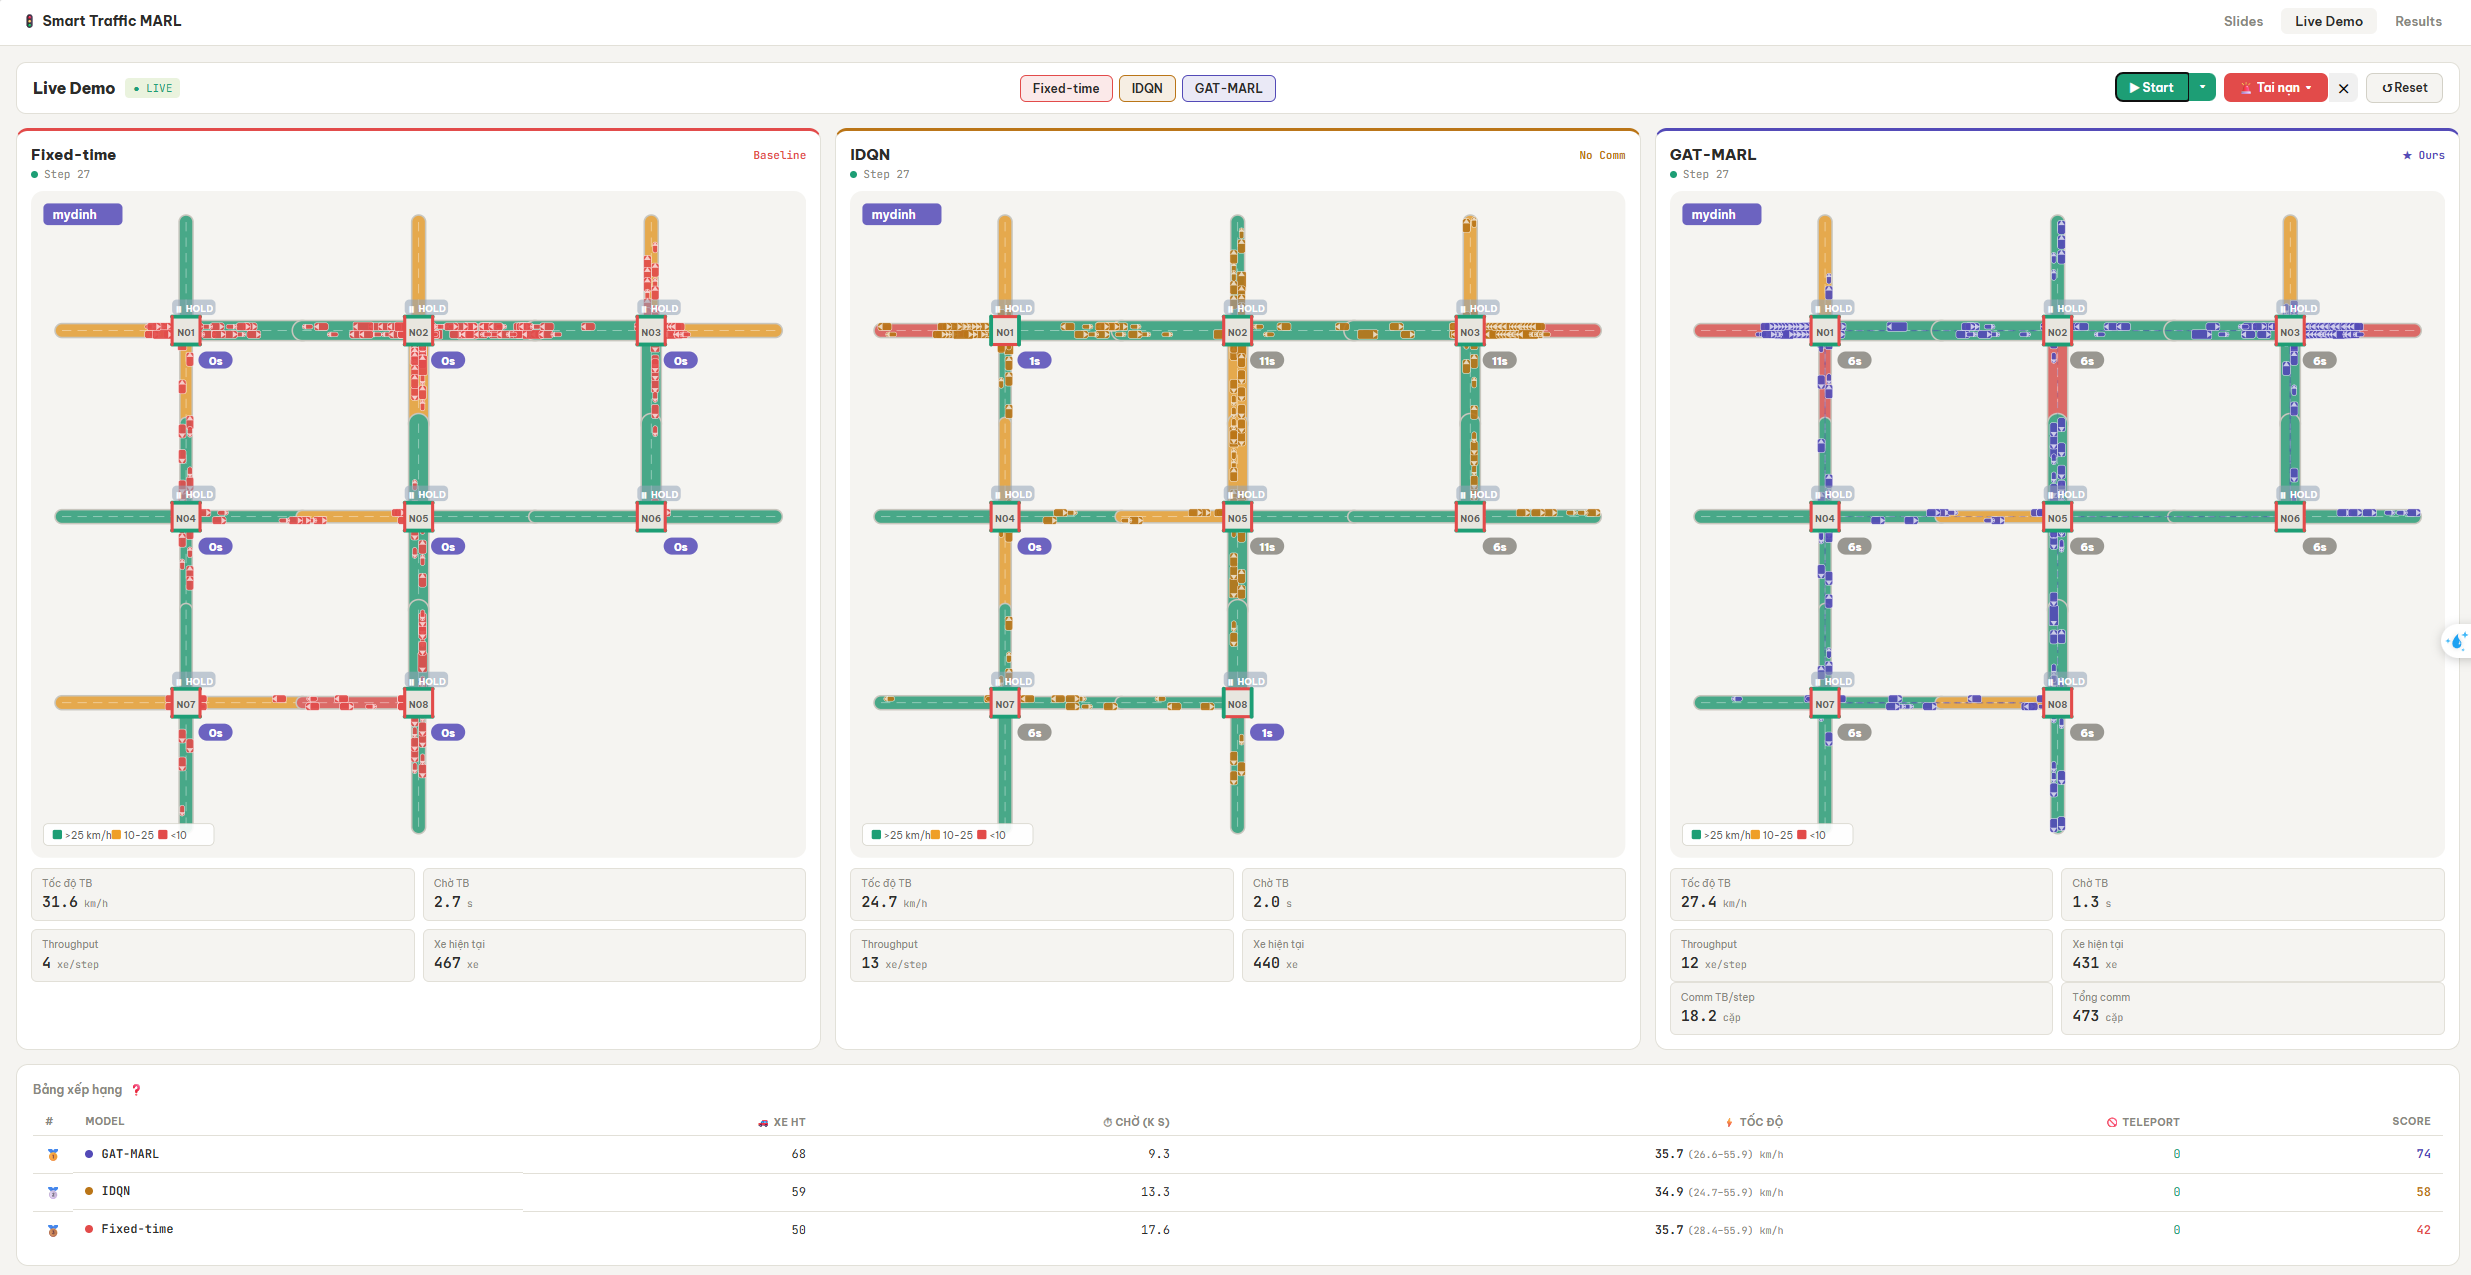
\includegraphics[width=0.9\linewidth,height=0.7\textheight,keepaspectratio]{imgs/live_demo_mydinh.png}
  \end{center}
  \vspace{0.2em}
  \small FastAPI + WebSocket backend / React + Vite frontend.
  So sánh trực tiếp Fixed-time, IDQN, GAT-MARL trên cùng episode.
\end{frame}

% ══════════════════════════════════════════════════════════════════════════════
\section{Thảo luận \& Kết luận}
% ══════════════════════════════════════════════════════════════════════════════

\begin{frame}{Thảo luận}
  \begin{columns}
    \column{0.5\textwidth}
      \textbf{Tại sao GAT thua IDQN ở Mỹ Đình?}
      \begin{enumerate}
        \item \textbf{Credit assignment} bất ổn:\\
              Hybrid reward + obstacle $\Rightarrow$ episodes "thảm họa"\\
              (min reward $= -1525$ vs $-882$ của IDQN)
        \item \textbf{Graph quá nhỏ} ($N=8$):\\
              4 heads dễ học pattern trùng lặp\\
              $\Rightarrow$ overfit, không generalize
      \end{enumerate}

    \column{0.5\textwidth}
      \textbf{GAT phát huy khi graph đủ lớn (UET):}
      \begin{itemize}
        \item Attention có ý nghĩa hơn trên 15 ngã tư
        \item Knowledge transfer hiệu quả qua 2-phase fine-tuning
      \end{itemize}
      \vspace{0.5em}
      \textbf{Hướng phát triển:}
      \begin{itemize}
        \item Prioritized experience replay
        \item Action space đa phase
        \item Mạng lưới $>$15 ngã tư
      \end{itemize}
  \end{columns}
\end{frame}

% ── Kết luận ──────────────────────────────────────────────────────────────────
\begin{frame}{Kết luận}
  \begin{block}{Đóng góp chính}
    \begin{itemize}
      \item \textbf{Reward hybrid} với normalization đảm bảo $\alpha{:}\beta = 70{:}30$ thực sự
      \item \textbf{Parallel training} Ape-X style với fixed-role epsilon workers
      \item \textbf{2-phase fine-tuning}: GAT-MARL finetune \textbf{200 ep} đạt kết quả tốt hơn IDQN train từ đầu \textbf{500 ep} --- ít tài nguyên hơn, hiệu quả hơn
      \item \textbf{Dashboard real-time} so sánh 3 phương pháp song song
    \end{itemize}
  \end{block}

  \vspace{0.5em}
  \begin{center}
    \large Cảm ơn thầy/cô và các bạn đã lắng nghe!\\[0.5em]
    \normalsize \texttt{\{24022397, 24022325, 24022355\}@vnu.edu.vn}\\
    \url{https://github.com/MinhCYB/Traffic-MARL}
  \end{center}
\end{frame}

% ══════════════════════════════════════════════════════════════════════════════
\end{document}